% !Mode\dots ``TeX:UTF-8''
\documentclass[serif]{beamer}
%\usetheme{Warsaw}
\usepackage{hyperref}
\usepackage{subcaption}
\usepackage{euscript}
%\usepackage{natbib}
\DeclareGraphicsExtensions{.png,.jpg}
\usepackage{default}


%自定义的宏
\include{def}
% 图片路径
\graphicspath{{img/}}
\title{BlockChain}
\subtitle{Bitcoin}
\author{ Liyun Dai}

\institute{RISE, Southwest University, Chongqing, China}
\date{\today}

\begin{document}
\maketitle
\begin{frame}
  \frametitle{Table of Contents}
  \tableofcontents[currentsection]
\end{frame}

\AtBeginSection[]
{\begin{frame}
	\frametitle{Table of Contents}
		\tableofcontents[currentsection]
\end{frame}}
\section{Introducing Bitcoin}

\begin{frame}{Market}
	
	\begin{figure}
		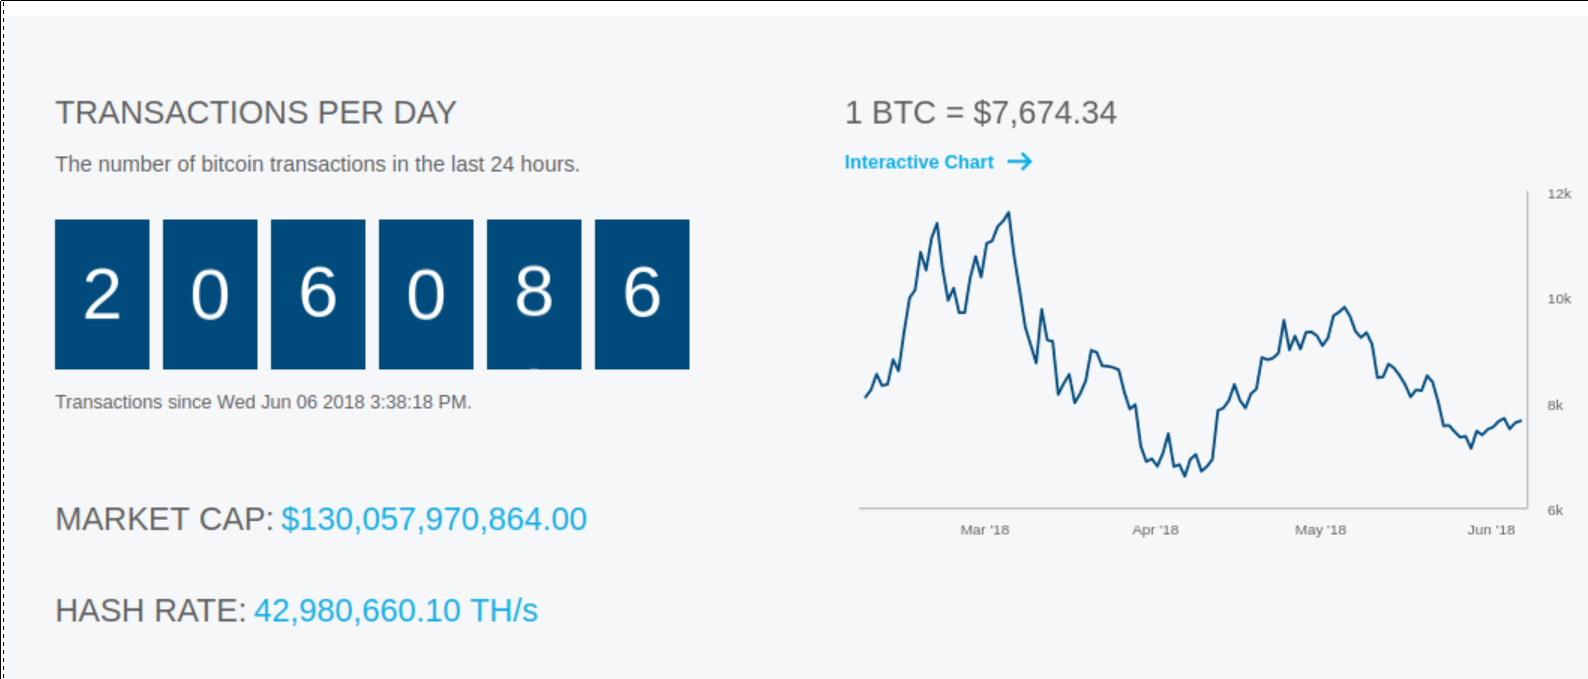
\includegraphics[width=0.8\textwidth]{bitcoin}
		\caption{2018.6.7}
		\label{fig:mark}
	\end{figure}
	
\end{frame}
\begin{frame}{Price}
	
	\begin{figure}
		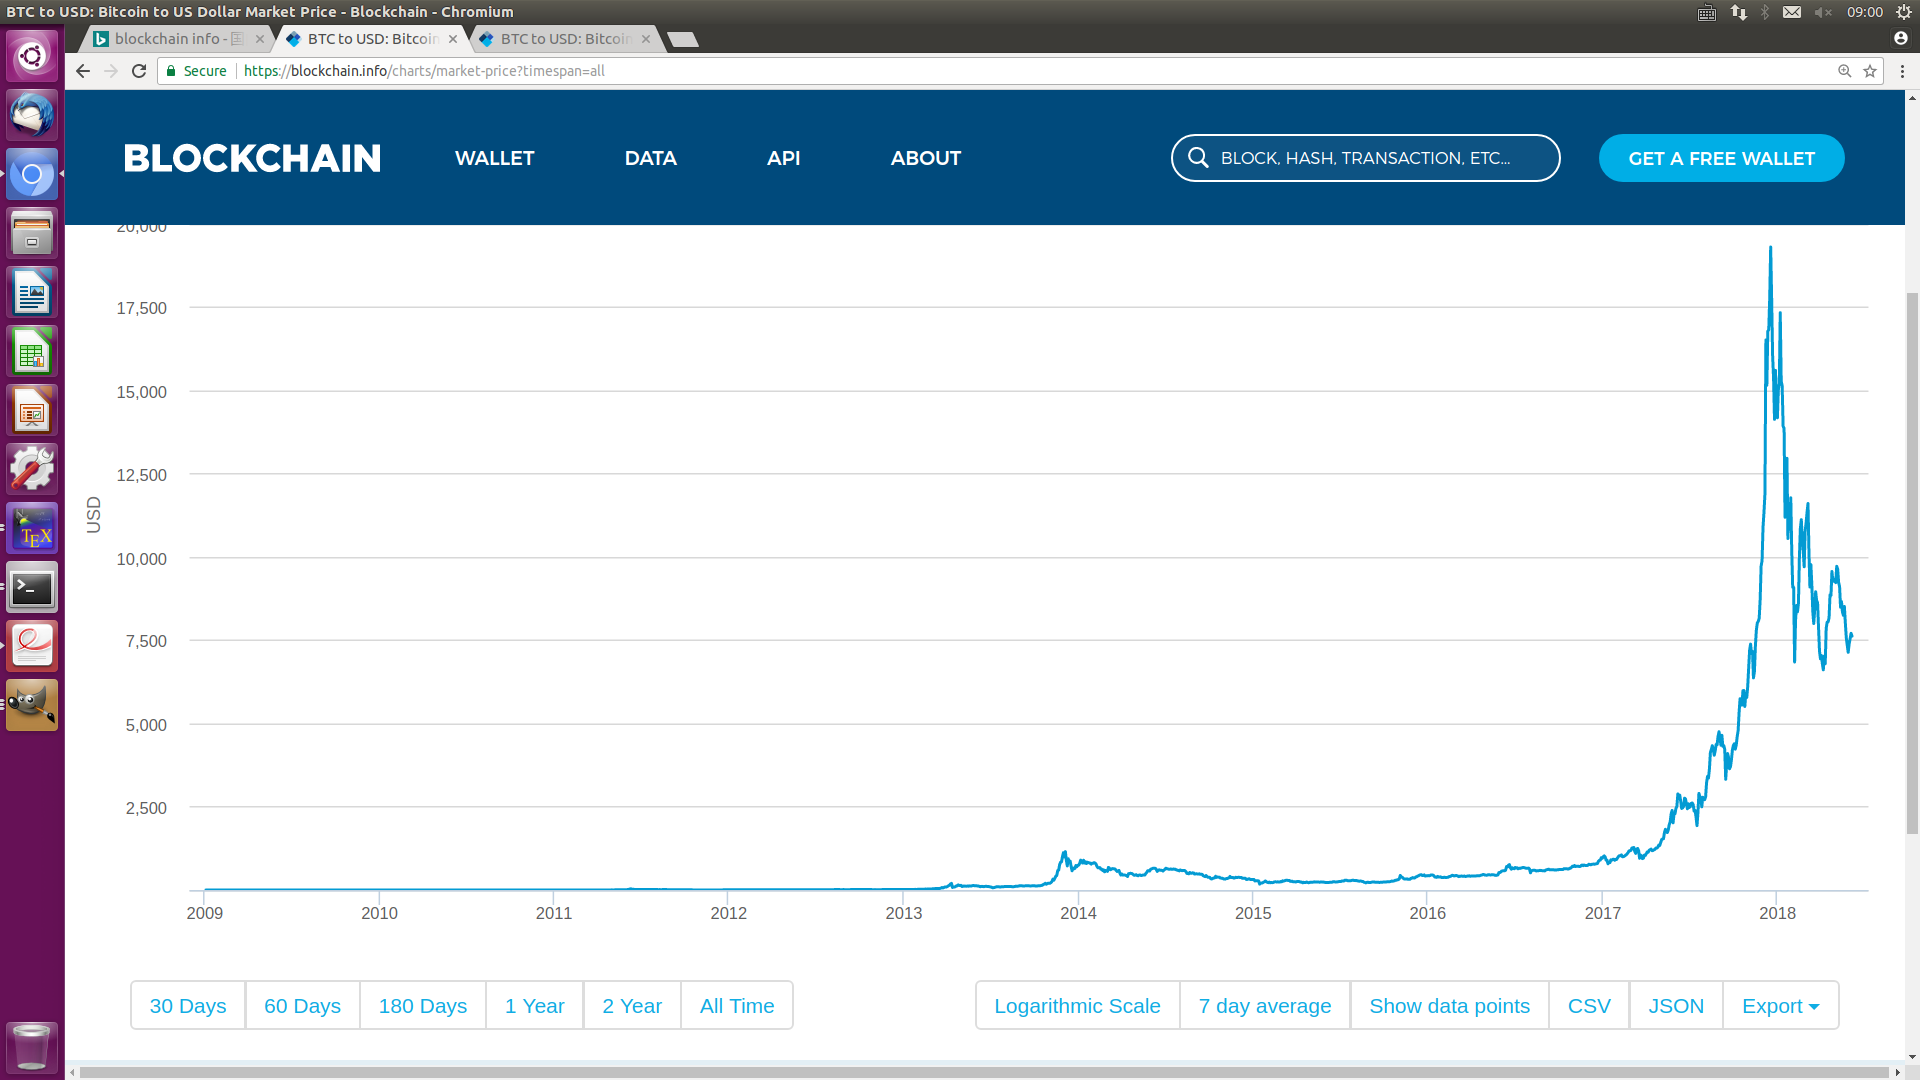
\includegraphics[width=0.9\textwidth]{price}
		\caption{2018.6.7}
		\label{fig:price}
	\end{figure}
	
\end{frame}
\begin{frame}{Bitcoin definition}
	\begin{definition}[Bitcoin]
			Bitcoin can be defined in various ways; it's a protocol, a digital currency, and a platform.
	\end{definition}
	It is a combination of
	\begin{enumerate}
		\item peer-to-peer network,
		\item protocols,
		\item  software that facilitate the creation.   
	\end{enumerate}

\end{frame}
\section{Bitcoin – a bird's-eye view}
\begin{frame}{Main components}
	\begin{enumerate}
		\item Digital keys
		\item Addresses
		\item Transactions
		\item Blockchain
		\item Miners
		\item The Bitcoin network
		\item Wallets (client software)
	\end{enumerate}
\end{frame}
\subsection{Sending a payment to someone}
\begin{frame}{Payment request is created}
		\begin{figure}
			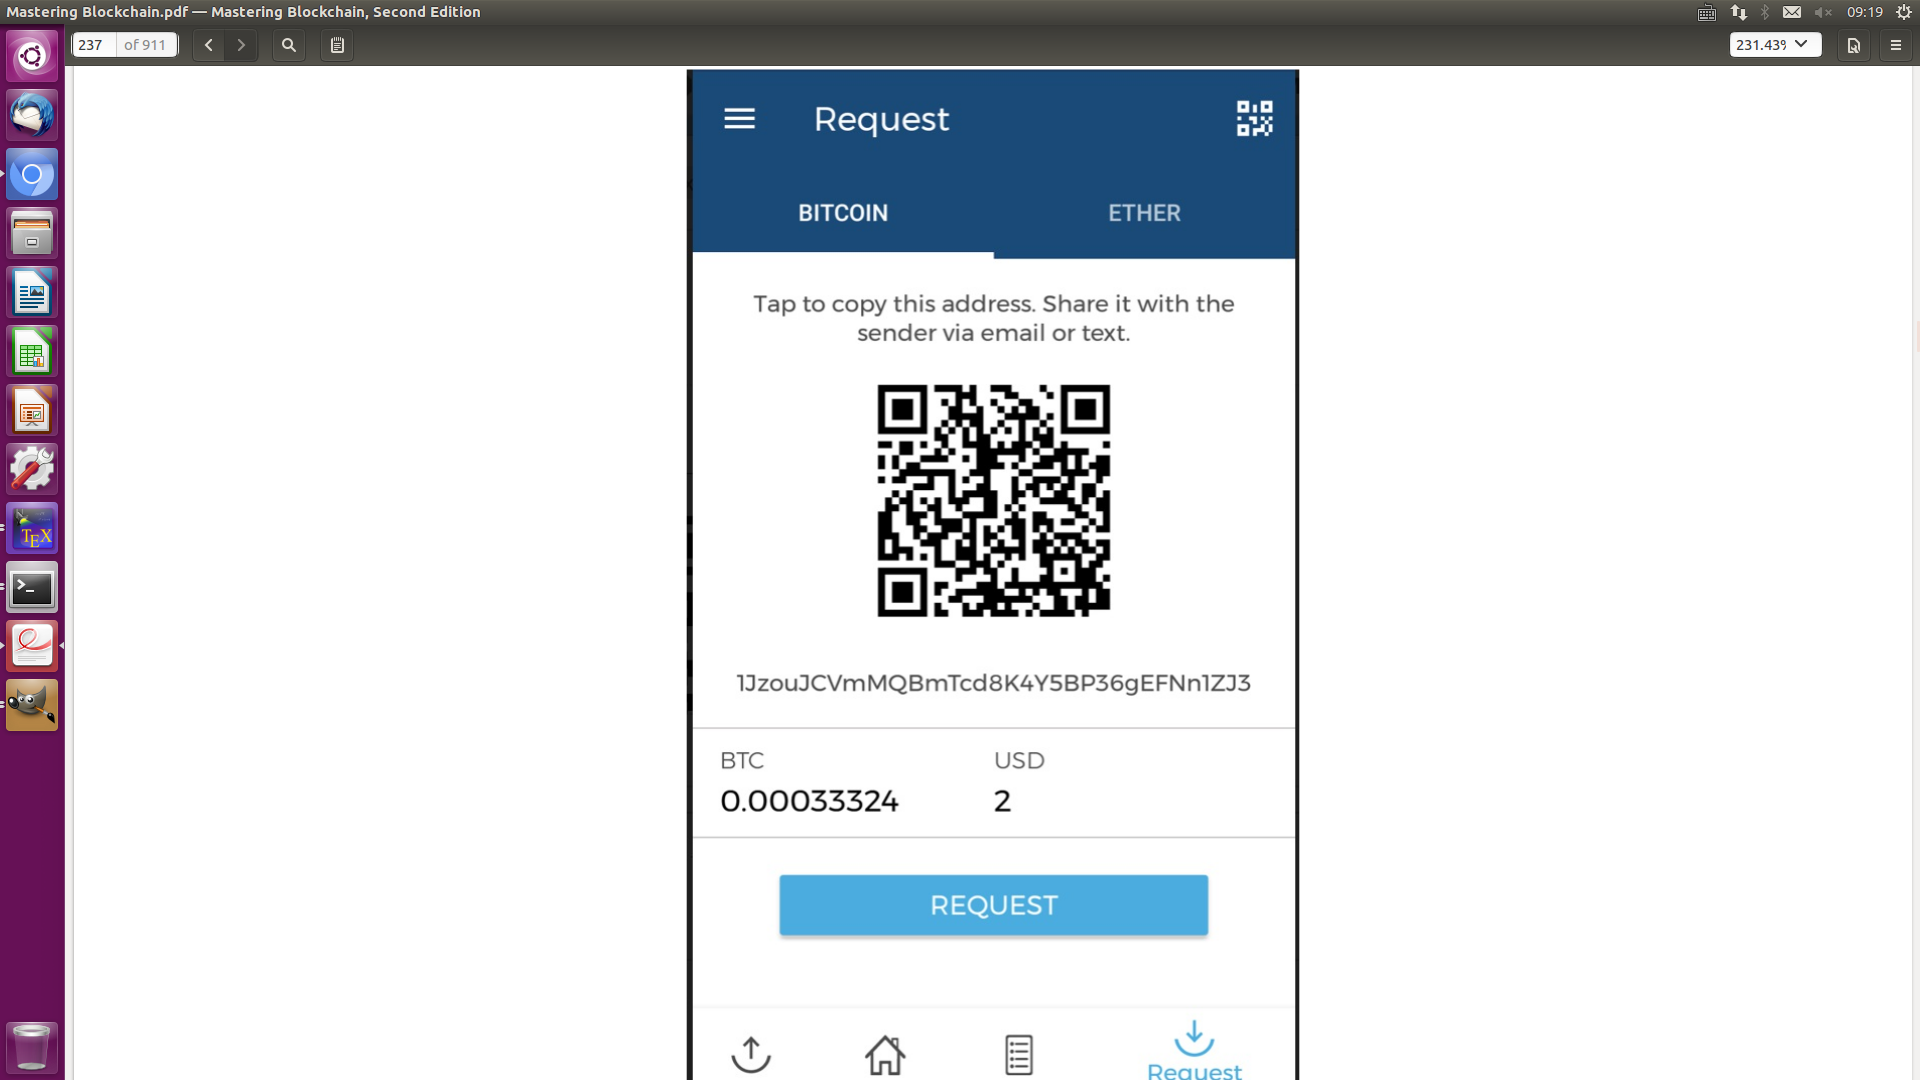
\includegraphics[width=0.9\textwidth]{request}
			\label{fig:request}
		\end{figure}
\end{frame}
\begin{frame}{Sender}
	\begin{figure}
		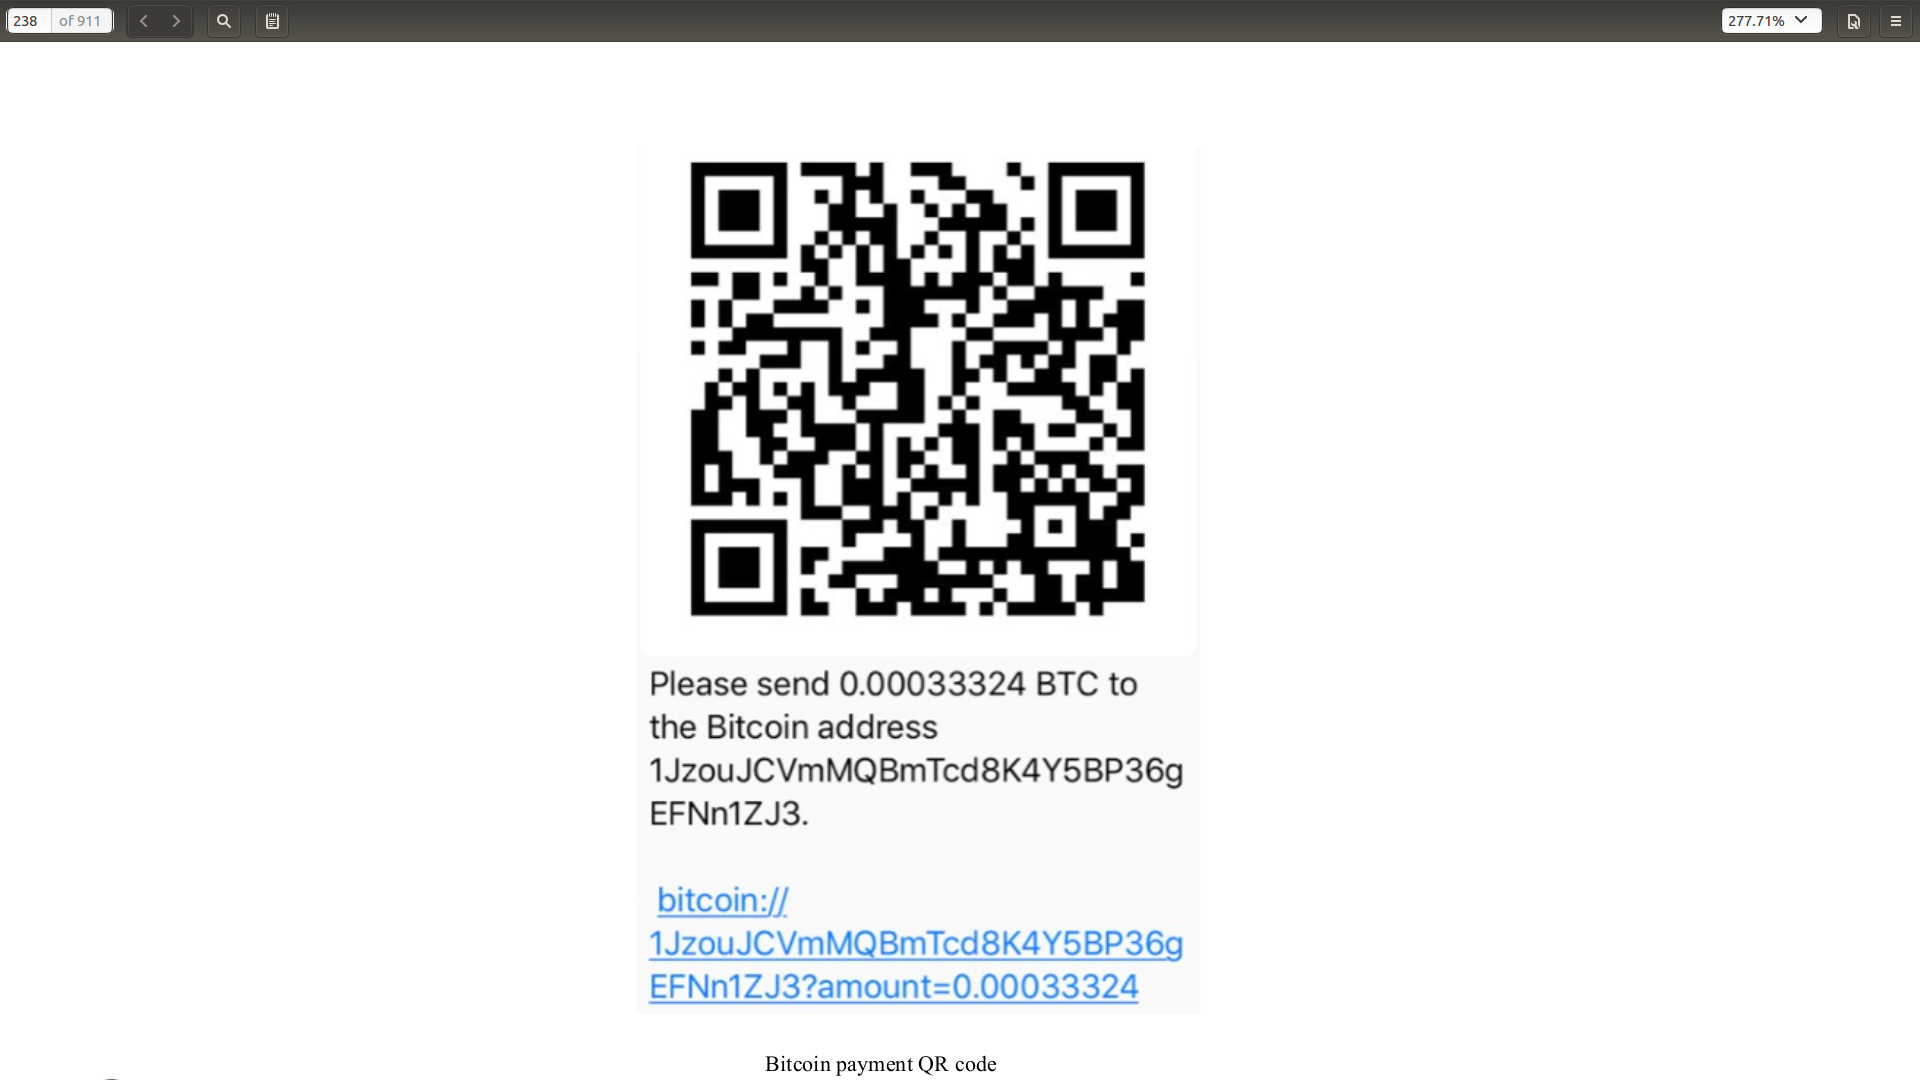
\includegraphics[width=0.9\textwidth]{sender}
		\label{fig:request2}
	\end{figure}
	
\end{frame}

\begin{frame}{Transaction creation}

		This transaction is digitally signed using the private key of the sender
		before broadcasting it.
			\begin{figure}
				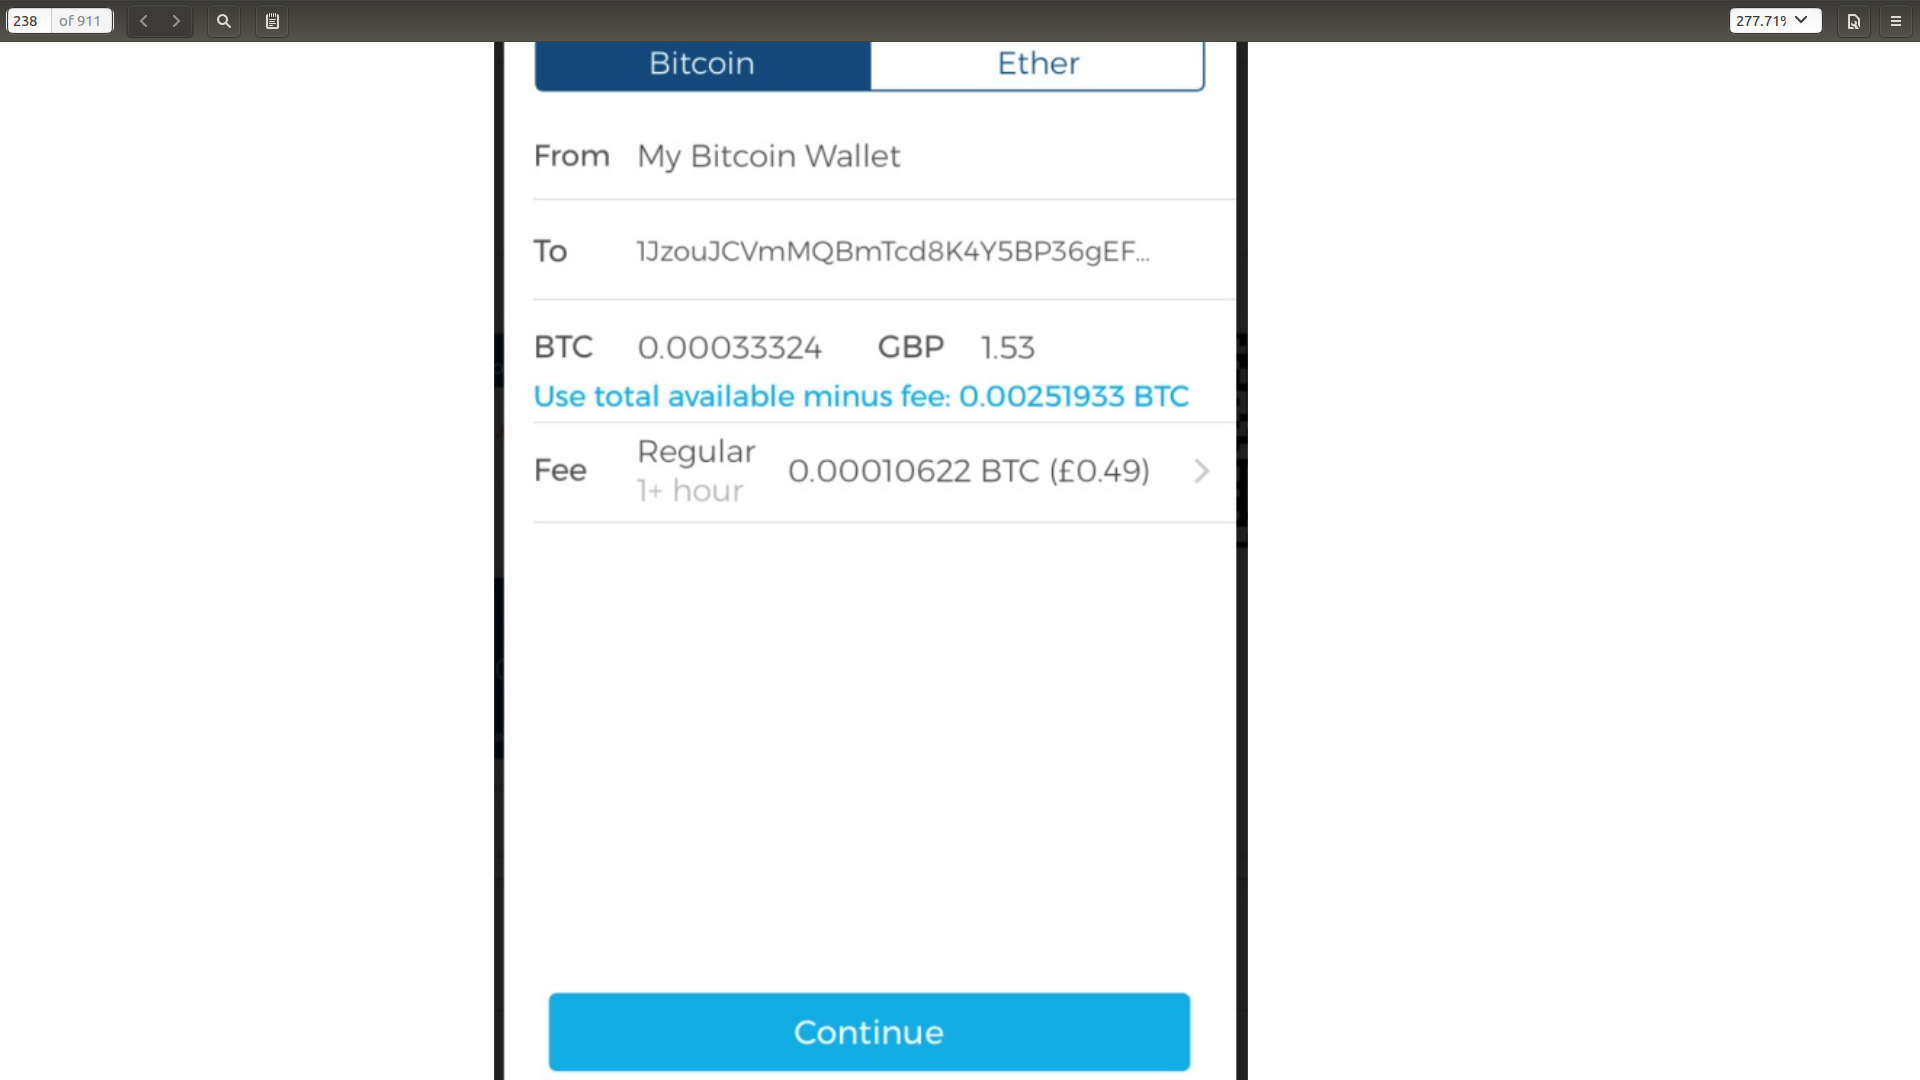
\includegraphics[width=0.9\textwidth]{result}
				\label{fig:result}
			\end{figure}

\end{frame}


\begin{frame}
	\begin{figure}
		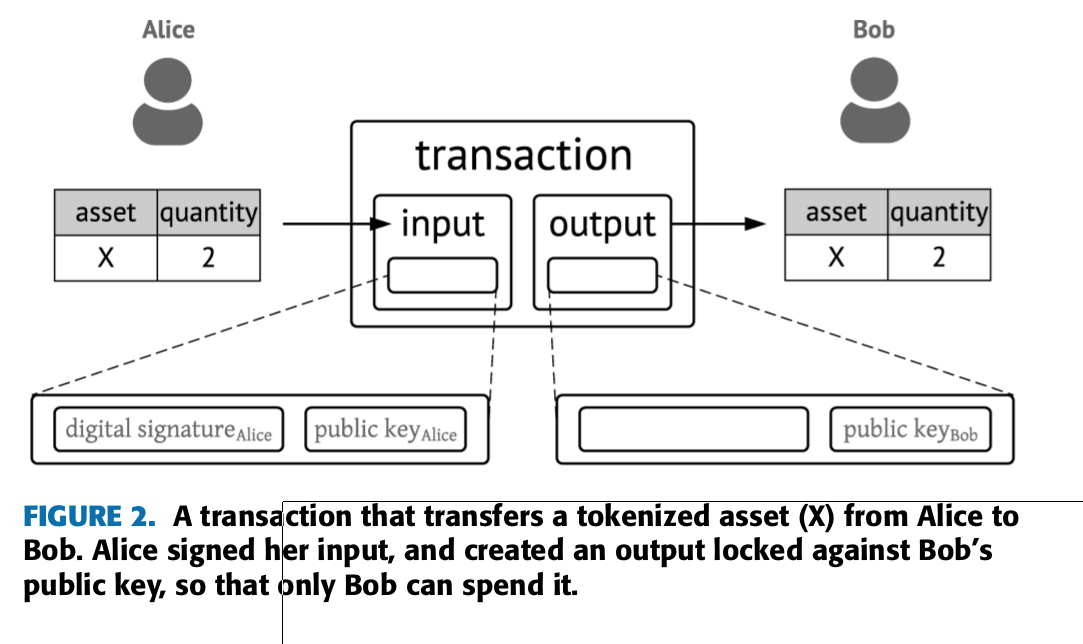
\includegraphics[width=0.9\textwidth]{trans}
		\label{fig:result10}
	\end{figure}
\end{frame}
	
	\begin{frame}{After sending (confirm)}
	
		\begin{figure}
			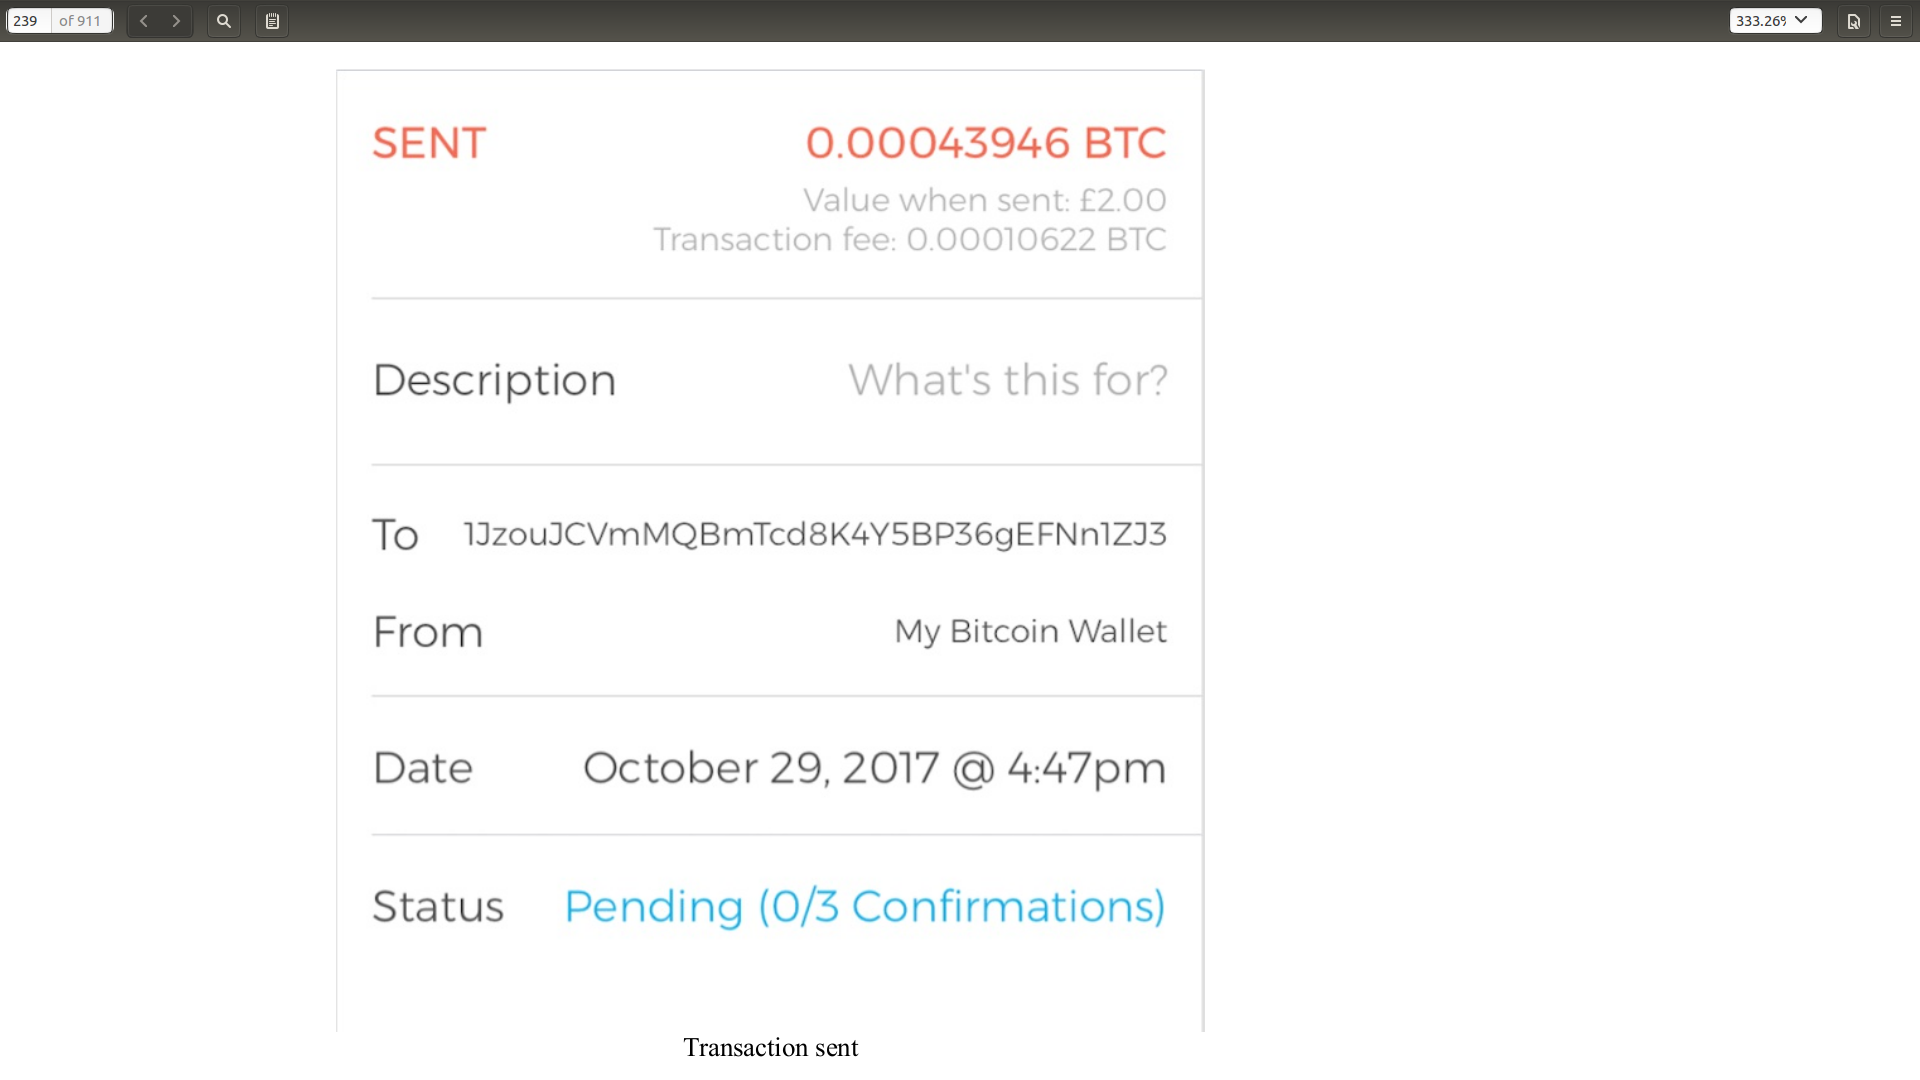
\includegraphics[width=0.9\textwidth]{after}
			\label{fig:result1}
		\end{figure}
		
	\end{frame}
	\begin{frame}{Transaction}
		In summary, the payment transaction in the Bitcoin network can be divided into the following steps:
		\begin{enumerate}[<+->]
			\item Transaction starts with a sender signing the transaction with their private key,
			\item Transaction is serialized so that it can be transmitted over the network,
			\item Transaction is broadcasted to the network,
			\item Miners listening for the transactions picks up the transaction,
			\item Transaction are verified for their validity by the miners,
			\item Transaction are added to the candidate/proposed block for mining,
			\item Once mined, the result is broadcasted to all nodes on the Bitcoin network.																																																								
		\end{enumerate}
	\end{frame}
	\section{Digital keys and addresses}
	\begin{frame}{PKC}
	Elliptic Curve Cryptography (ECC) is used to generate public and private key pairs in the Bitcoin network.
	\end{frame}
	\begin{frame}{Private key}
		Private keys are fundamentally 256-bit numbers randomly chosen in the range specified by the secp256k1 ECDSA
		curve recommendation. {\color{red}{Any randomly chosen}} 256-bit number from 0x1 to 0xFFFF FFFF FFFF FFFF FFFF FFFF FFFF FFFE
		BAAE DCE6 AF48 A03B BFD2 5E8C D036 4140 is a valid private key.
		\begin{example}
			The following is an example of a private key:
			{\tiny A3ED7EC8A03667180D01FB4251A546C2B9F2FE33507C68B7D9D4E1FA5714195201}
		\end{example}
	\end{frame}
	\begin{frame}{Public keys in Bitcoin}
		Public keys exist on the blockchain and {\color{red}{all network participants}} can see it.  Once a transaction signed with the
		private key is broadcasted on the Bitcoin network, public keys are used by the nodes to verify that the
		transaction has indeed been signed with the corresponding private key. This process of verification proves the
		{\color{red}{ownership}} of the bitcoin.
	\end{frame}
	\begin{frame}{Addresses in Bitcoin}
		A bitcoin address is created by taking the corresponding public key of a private key and hashing it twice, first
		with the SHA-256 algorithm and then with RIPEMD-160. The resultant 160-bit hash is then prefixed with a
		version number and finally encoded with a Base58Check encoding scheme. The bitcoin addresses are 26-35
		characters long and begin with digit 1 or 3.
		\begin{example}
			1ANAguGG8bikEv2fYsTBnRUmx7QUcK58wt
		\end{example}
	\end{frame}
	

	
	\begin{frame}{Network}
		\begin{enumerate}[<+->]
			\item New transactions are broadcast to all nodes.
			\item Each node collects new transactions into a block.
			\item Each node works on finding a difficult proof-of-work for its block.
			\item When a node finds a proof-of-work, it broadcasts the block to all nodes.
			\item Nodes accept the block only if all transactions in it are valid and not already spent.
			\item Nodes express their acceptance of the block by working on creating the next block in the
			chain, using the hash of the accepted block as the previous hash.
		\end{enumerate}
		
	\end{frame}
		\begin{frame}{Confirm (Proof-of-Work)}
			\begin{figure}
				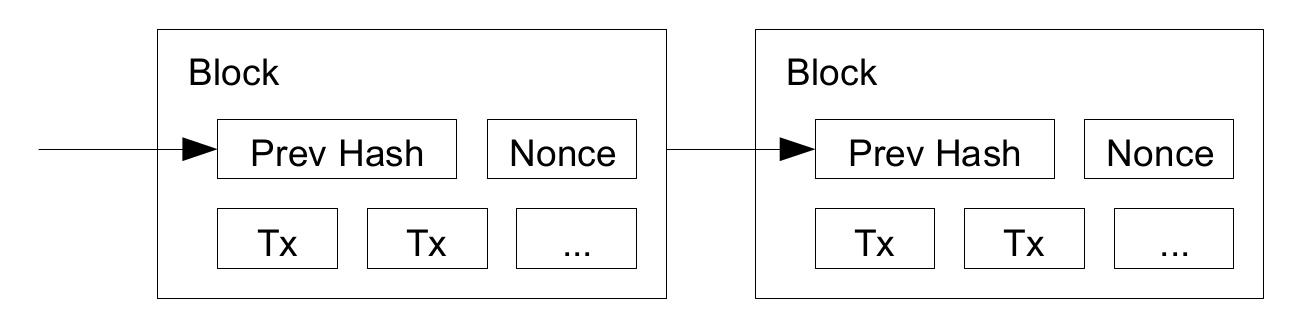
\includegraphics[width=0.6\textwidth]{proof}
				\label{fig:result3}
			\end{figure}
			Repeatedly choose value  of {\tt Nonce} make the {\tt HASH-256} of corresponding block satisfy 
			condition.
			\begin{example}
				\begin{figure}
					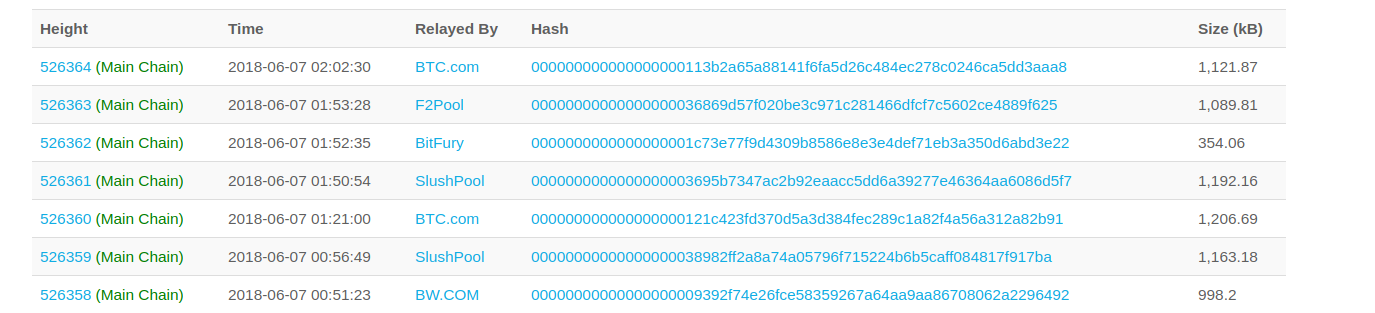
\includegraphics[width=0.75\textwidth]{example1}
					\label{fig:result4}
				\end{figure}
			\end{example}
			
		\end{frame}
	\begin{frame}{The cost of mining(1)}
		Average computing $16^{18}=4722366482869645213696$ time {\tt HASH-256} can obtain a value which satisfies the condition.
		\begin{example}	
			Intel(R) Core(TM) i5-7400 CPU @ 3.00GHz
			1000 time takes $4.7$s.	
		\end{example}
			The Power consumption of  i5-7400  is 65W. Hence the average power take  i5-7400 create a 
			block is $$\frac{4722366482869645213696\times 4.6\times 65}{1000\times 4\times 3600\times 1000}\sim 9.8*10^{13} KW/H$$
			
	\end{frame}
	\begin{frame}{The cost of mining(2)}
			\begin{figure}
				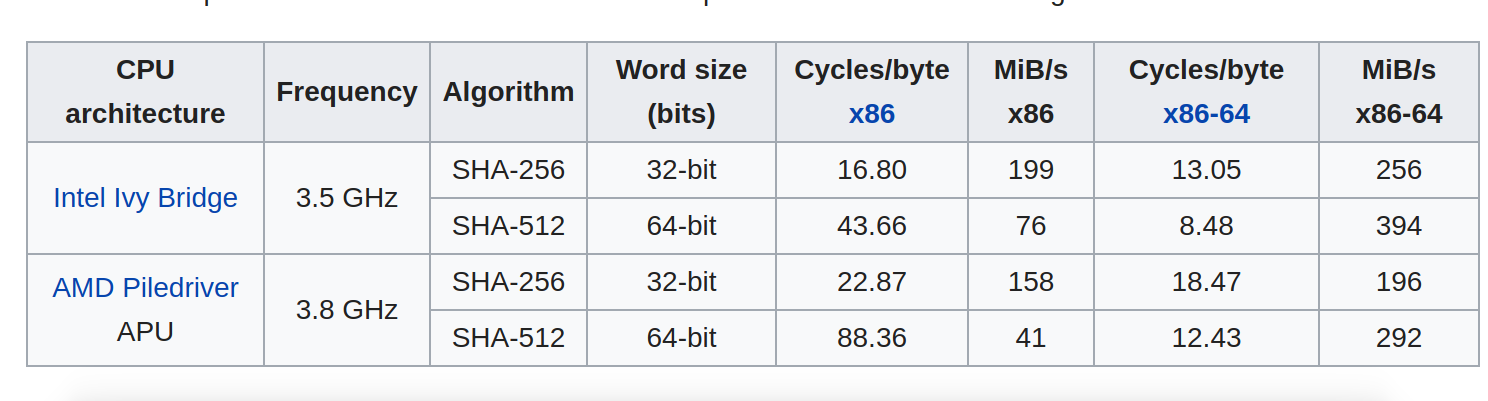
\includegraphics[width=0.9\textwidth]{perf}
				\label{fig:result5}
			\end{figure}
	\end{frame}
\end{document}